\chapter*{\texorpdfstring{绪论 \quad 实数}{绪论 实数}}

\section{有理数域}

\subsection{前言} \label{subsec:1}

从小学开始, 我们便很熟悉有理数及其性质了.
到了中学, 根式的引入使我们扩大了数的领域.
例如 $\sqrt{2}$ 就在我们所熟知的有理数中不存在.
也就是说, {\kaishu 并不存在这样的有理数 $\dfrac{p}{q}$ (式中 $p$ 和 $q$ 都是自然数),
其平方能等于 $2$}.

为了证明, 我们使用反证法:
设存在分数 $\dfrac{p}{q}$, 其平方 $\brac{\dfrac{p}{q}}^2 = 2$.
为了方便讨论, 我们可以假设 $\dfrac{p}{q}$ 是既约分数, 即 $p$ 和 $q$ 互质.
由于 $p^2 = 2q^2$, 则 $p$ 为偶数, 于是 $q$ 为奇数, 我们设 $p = 2r$ ($r$ 为整数).
用 $p$ 的式子代入, 得 $q^2 = 2r^2$, 由此推得 $q$ 为偶数.
所得的矛盾便证明了我们的命题.

在几何学上, 若我们仅停留在有理数的范围内, 那么并非一切的线段都能有一个\emph{长度}.
例如, 考察边长为单位长度的正方形.
依勾股定理, 其对角线长度的平方应等于 $2$, 上面我们已经证过, 这不可能为有理长度 $\dfrac{p}{q}$.

所以, 无论是在代数还是几何上, 我们的有理数都显得不太够用,
为了解决类似的情况, 我们将在本绪论中为有理数域添上一种新的数,
称为无理数, 用以扩大有理数域的范围.
同时, 我们将证明, 对有理数施行算术运算及用等号、不等号把它们连接起来等众所周知的性质,
在这个扩大的领域内仍然是正确的.
为了对扩大后的数域验证上述性质, 需选出为数最少的几个\emph{基本性质},
只要它们成立, 其余的一切性质都能作为形式逻辑的结果而从之推出了.

因此, 我们下面先总结有理数域的一些基本性质.
我们这里所说的“数”, 总是指有理数, 习惯上用字母 $a, b, \cdots$ 等来表示它们.

\subsection{有理数域的序} \label{subsec:2}

首先让我们约定: “相等”($=$) 代表了等号左右两边同一种概念的不同形式,
二者可以随意替换, 在数学意义上没有任何区别.
它的性质是平凡的, 没有什么可研究的.
我们更关心的是“不等”的情况, 这被称作\emph{序}\index{xu@序}.

有理数域的序得自“大于”($>$)的概念, 与之有关的是第一组性质:
{\kaishu
    \myrefparagraph{I $1^\circ$}\label{ax:rational_order_1}
    每一对数 $a$ 与 $b$ 之间必有且仅有下列关系之一:
    $$
    a = b, \quad a > b, \quad a < b;
    $$

    \myrefparagraph{I $2^\circ$}\label{ax:rational_order_2}
    由 $a > b$ 及 $b > c$ 可推得 $a > c$ ($>$ 的传递性);

    \myrefparagraph{I $3^\circ$}\label{ax:rational_order_3}
    若 $a > b$, 则必能求得一数 $c$, 使
    $$a > c, \quad \text{且} \quad c > b
    \ \footnote{在这条件下也说成: 数 $c$ 位于数 $a$ 与 $b$ 之间. 显然, 这样的数有无限个之多.}
    \ \text{(\emph{稠密性}\index{youlishudechoumixing@有理数的稠密性})}.$$
}

“小于”($<$)的概念则是作为“大于”的派生而引入.
说 $a < b$, 就是等价于说 $b > a$.
显而易见, \ref{ax:rational_order_2} 和 \ref{ax:rational_order_3}
所代表的性质 “小于” 同样满足.

\subsection{有理数的加法及减法} \label{subsec:3}

第二组性质是关于加法的, 即关于求两数之和的运算性质.
对于每一对数 $a$ 及 $b$, 存在着一个唯一的数,
被称为 $a$ 与 $b$ 的\emph{和}\index{youlishudehe@有理数的和} (记成 $a + b$).
这概念具有下列的性质:

{\kaishu
    \myrefparagraph{II $1^\circ$}\label{ax:rational_add_1}
    $a + b = b + a$ (加法的交换律);

    \myrefparagraph{II $2^\circ$}\label{ax:rational_add_2}
    $\brac{a + b} + c = a + \brac{b + c}$ (加法的结合律).
}

“$0$” 这个数比较特殊, 它具有下列特性:

{\kaishu
    \myrefparagraph{II $3^\circ$}\label{ax:rational_add_3} $a + 0 = a$;
}\\
此外,
{\kaishu
    \myrefparagraph{II $4^\circ$}\label{ax:rational_add_4}
    对每一数 $a$ 存在着与它相反的数 $-a$, 使 $a + \brac{-a} = 0$.
}

在这些性质的基础上, 首先可以解决加法的逆运算即\emph{减法}的问题.
通常称使 $c + b = a$
\footnote{依 \ref{ax:rational_add_1}, 定义差的等式可写成: $b + c = a$.}
的数 $c$, 为数 $a$ 及 $b$ 的\emph{差}\index{youlishudecha@有理数的差}.
伴随而来的问题就是: 这样的数是否存在? 如果存在, 是否唯一?

为说明这一点, 我们
    设 $c = a + \brac{-b}$, 则根据 [\ref{ax:rational_add_2}, \ref{ax:rational_add_1}, \ref{ax:rational_add_4}, \ref{ax:rational_add_3}], 有
    $$
    c + b = \bbrac{a + \brac{-b}} + b = a + \bbrac{\brac{-b} + b} = a + \bbrac{b + \brac{-b}} = a + 0 = a.
    $$
    因此, 这 $c$ 满足于差的定义, 其存在性得证.

    为了证明唯一性, 我们利用反证法.
    假设还有一数 $c'$ 也为 $a$ 及 $b$ 的差, 即有 $c' + b = a$.
    在这等式两边各加 $\brac{-b}$, 并变换其左边 [\ref{ax:rational_add_2}, \ref{ax:rational_add_4}, \ref{ax:rational_add_3}]:
    $$
    \brac{c' + b} + \brac{-b} = c' + \bbrac{b + \brac{-b}} = c' + 0 = c',
    $$
    结果得 $c' = a + \brac{-b} = c$.
    这样就证明了这个数的唯一性.

    这样, 我们就证明了数 $a$ 及 $b$ 的差的存在及唯一性, 可以把它记成 $a - b$.

由差的唯一性可以推得一系列的推论.
第一, 由 \ref{ax:rational_add_3} 推得 $0 = a - a$, 因而得出结论:
除去数 $0$ 以外, 不存在具有性质 \ref{ax:rational_add_3} 的其他数.
第二, 由 $-a = 0 - a$ 可推得所给数的相反数是唯一的.

因为由 $a + \brac{-a} = 0$ 可推得 $\brac{-a} + a = 0$ [\ref{ax:rational_add_1}],
所以 $a = -\brac{-a}$, 即数 $a$ 和 $-a$ 互为相反数.
我们再来证明相反数满足下述性质:
$$
-\brac{a + b} = \brac{-a} + \brac{-b}.
$$
为此, 只需证明
$$
\brac{a + b} + \bbrac{\brac{-a} + \brac{-b}} = 0,
$$
而这由 \ref{ax:rational_add_1}, \ref{ax:rational_add_2}, \ref{ax:rational_add_4}, \ref{ax:rational_add_3} 便可推得.

最后, 再引进联系 $>$ 与加号的一个性质:
{\kaishu
    \myrefparagraph{II $5^\circ$}\label{ax:rational_add_5} 由 $a > b$ 可推得 $a + c > b + c$.
}

它使我们得以在不等式的两边各加上一个等量, 用它又可证明两不等式
$$
a > b \quad \text{和} \quad a - b > 0
$$
是等价的.
然后, 由 $a > b$ 得 $a - b > 0$, 而
$a - b = a + \brac{-b} = \brac{-b} + a = \brac{-b} + \bbrac{-\brac{-a}} = \brac{-b} - \brac{-a}$,
因此这不等式可改写成 $\brac{-b} - \brac{-a} > 0$, 由此 $-b > -a$ 或 $-a < -b$.
即{\kaishu 由 $a > b$ 可推得 $-a < -b$}.

特别地, 由 $a > 0$ 可推得 $-a < 0$, 由 $a < 0$ 可推得 $-a > 0$.
若 $a \neq 0$, 则在两个相反的数 $a$ 及 $-a$ 中, 必有且仅有一个大于 $0$ 的数, 我们把它称为数 $a$ 或数 $-a$ 的\emph{绝对值}\index{youlishudejueduizhi@有理数的绝对值}, 记成
$$
\abs{a} = \abs{-a}.
$$
我们规定, 零的绝对值就定为零: $\abs{0} = 0$.

根据性质 \ref{ax:rational_add_5}, 由 $a > b$ 可推得 $a + c > b + c$;
仿此, 由 $c > d$ 可推得 $c + b > d + b$, 或根据 \ref{ax:rational_add_1} 有 $b + c > b + d$,
最后由 \ref{ax:rational_order_2} 可得 $a + c > b + d$.
这就是不等式的边边相加: {\kaishu 由 $a > b$ 及 $c > d$ 可推得 $a + c > b + d$}.

\subsection{有理数的乘法及除法} \label{subsec:4}

第三组性质是关于乘法的, 即关于求两数之积的运算性质.
对于每一对数 $a$ 及 $b$ 存在着一个唯一的数, 被称为 $a$ 与 $b$ 的\emph{积}\index{youlishudeji@有理数的积}(记成 $a \cdot b$ 或 $ab$).
这概念具有下列性质:
{\kaishu
    \myrefparagraph{III $1^\circ$}\label{ax:rational_mul_1} $ab = ba$ (乘法的交换律);
    \myrefparagraph{III $2^\circ$}\label{ax:rational_mul_2} $\brac{ab}c = a\brac{bc}$ (乘法的结合律).
}

“$1$” 这个数比较特殊, 它具有下列特性:
{\kaishu
    \myrefparagraph{III $3^\circ$}\label{ax:rational_mul_3} $a \cdot 1 = a$;
}\\
此外,
{\kaishu
    \myrefparagraph{III $4^\circ$}\label{ax:rational_mul_4} 对于每一异于 $0$ 的数 $a$, 必有数 $\dfrac{1}{a}$ (其倒数), 使 $a \cdot \dfrac{1}{a} = 1$.
}

正如前面根据加法的性质来解决关于减法的问题一样, \emph{除法}, 作为乘法的逆运算, 亦可根据乘法的性质来解决.
倒数在这里的作用正如相反数在那里的作用一样.

如果一数 $c$ 满足关系
$$
c \cdot b = a
\ \footnote{依 \ref{ax:rational_mul_1}, 定义商的这个等式也可写成: $b \cdot c = a$.}
$$
(其中除数 $b$ 常预先假定异于 $0$), 则 $c$ 称为 $a$ 及 $b$ 的\emph{商}\index{youlishudeshang@有理数的商}.
因 [\ref{ax:rational_mul_2}, \ref{ax:rational_mul_1}, \ref{ax:rational_mul_4}, \ref{ax:rational_mul_3}]
$$
\brac{a \cdot \frac{1}{b}} \cdot b = a \cdot \brac{\frac{1}{b} \cdot b} = a \cdot \brac{b \cdot \frac{1}{b}} = a \cdot 1 = a,
$$
那么, 令 $c = a \cdot \dfrac{1}{b}$, 就可以满足商的定义.

同样, 若数 $c'$ 也满足数 $a$ 及 $b$ 的商的定义, 于是 $c' \cdot b = a$, 则在这等式两边乘以 $\dfrac{1}{b}$, 并变换左边 [\ref{ax:rational_mul_2}, \ref{ax:rational_mul_4}, \ref{ax:rational_mul_3}]:
$$\brac{c' \cdot b} \cdot \frac{1}{b} = c' \cdot \brac{b \cdot \frac{1}{b}} = c' \cdot 1 = c', $$
就得到 $c' = a \cdot \dfrac{1}{b} = c$.

这样, 就证明了数 $a$ 与 $b$ (设 $b \neq 0$) 的商的存在及唯一性, 把它记成 $a \div b$ 或 $\dfrac{a}{b}$.
由商的唯一性可知, 除了 $1$ 以外, 再没有什么数能具有类似于 \ref{ax:rational_mul_3} 的性质.
由此, 如前所述, 也可推得倒数(看成 $1$ 及 $a$ 的商)的唯一性;
此外, 也容易证明数 $a$ 及 $\dfrac{1}{a}$ 互为倒数.

下列性质与加法及乘法都有关系:
{\kaishu
    \myrefparagraph{III $5^\circ$}\label{ax:rational_mul_5} $\brac{a + b}c = a \cdot c + b \cdot c$ (乘法关于和的分配律).
}

由此很易导出关于{\kaishu 乘法关于差的分配律}:
$$
\brac{a - b} \cdot c = a \cdot c - b \cdot c.
$$
依差的定义, 上式可直接由下式推出:
$$
\brac{a - b} \cdot c + b \cdot c = \bbrac{\brac{a - b} + b} \cdot c = a \cdot c.
$$

再应用性质 [\ref{ax:rational_add_3}] 和 \ref{ax:rational_mul_5}, 有
$$
a + 0 = a, \quad \brac{a + 0} \cdot b = a \cdot b + 0 \cdot b = a \cdot b,
$$
于是可推得 $0 \cdot b = 0$, 再由 \ref{ax:rational_mul_1} 得 $b \cdot 0 = 0$.
反之, 若 $a \cdot b = 0$ 且 $b \neq 0$, 则必须 $a = 0$.

最后我们指出联系符号 $>$ 与乘号的一个性质:
{\kaishu
    \myrefparagraph{III $6^\circ$}\label{ax:mul_6} 由 $a > b$ 及 $c > 0$ 可推得 $a \cdot c > b \cdot c$.
}

据此可以用正数乘不等式的两边.
由此可知, 当 $a > 0$ 及 $b > 0$ 时, 亦必有 $a \cdot b > 0$.

注意, $\brac{-a} \cdot b = -\brac{a \cdot b}$, 这可由下面推得
$$
a \cdot b + \brac{-a} \cdot b = \bbrac{a + \brac{-a}} \cdot b = 0 \cdot b = 0.
$$
现在不难看出, 若 $a < 0, b > 0$, 则 $a = -\abs{a}, b = \abs{b}$, 从而
$$
a \cdot b = \brac{-\abs{a}} \cdot \abs{b} = -\brac{\abs{a} \cdot \abs{b}} < 0;
$$
当 $a > 0, b < 0$ 时亦如此, 又若 $a < 0, b < 0$, 则
$$
a \cdot b = \brac{-\abs{a}} \cdot \brac{-\abs{b}} = -\bbrac{\abs{a} \cdot \brac{-\abs{b}}} = -\bbrac{-\brac{\abs{a} \cdot \abs{b}}} = \abs{a} \cdot \abs{b} > 0.
$$

这样, 我们已完全重新建立了关于乘法的符号规则, 这些符号规则现在已成为有理数的上述性质的逻辑推论了.
换言之, 如果有理数要满足上述诸性质, 就必定要遵守这些符号规则.
关于乘以 $0$ 的规则, 也可以这样说.

在处理了加法和乘法的性质以后, 我们现在能够证明在前面数的基本性质 [\ref{ax:rational_order_3}] 中已述及的有理数域的稠密性了.
例如, 由 $a > b$ 可推得 $a > \dfrac{a+b}{2} > b$.

\subsection{阿基米德公理} \label{subsec:5}
\index{ajimidegongli@阿基米德公理}

我们用下列简单而重要的论证, 来结束我们的有理数基本性质一览表.
这一性质是不能由上述的诸性质里推得的.
{\kaishu
    \myrefparagraph{IV $1^\circ$}\label{ax:archimedes} 不论 $c > 0$ 是怎样的数, 总有大于 $c$ 的自然数 $n$ 存在着.
}

实际上, 阿基米德曾说明了一个几何命题:
{\kaishu
若在直线上给定任意两线段 $A$ 及 $B$, 则 $A$ 重复相加若干次后, 其和总可以大于 $B$:
$$
\underbrace{A + A + \cdots + A}_{n \text{次}} = A \cdot n > B.
$$
}

若将这论证转而对正数 $a$ 及 $b$ 来叙述, 它便肯定有这样的自然数 $n$ 存在使
$$\underbrace{a + a + \cdots + a}_{n \text{次}} = a \cdot n > b.$$

若应用已研究过的有理数的性质, 则这不等式相当于 $n > \dfrac{b}{a}$, 把商 $\dfrac{b}{a}$ 记成 $c$, 我们便得出上面所叙述的 \ref{ax:archimedes}.

\section{\texorpdfstring{无理数的导入 $\cdot$ 实数域的序}{无理数的导入·实数域的序}}

\subsection{无理数的定义} \label{subsec:6}

将有理数集及其在第一节内列举的一切性质作为已知前提, 下面我们仿效 Dedekind 来叙述无理数的理论
\footnote{也可以把实数的基本性质直接作为公理而不加证明地承认. 采用这种公理化途径的读者, 可以跳过本节的具体构造, 从第 \ref{subsec:10}、\ref{subsec:11} 节继续阅读.}.
有理数域内的分划概念是这套理论的基础.
若将全体有理数构成的集合划分为两个非空集合 $A$ 与 $A'$ (即每个集合都至少包含一个元素),
只要满足以下条件, 我们就把这样的划分称为\emph{分划}\index{fenhua@分划}:
{\kaishu
    \myrefparagraph{1$^\circ$}\label{ax:rational_cut_1} 任意有理数, 必在且仅在 $A$ 与 $A'$ 这两个集合之一中出现
    \footnote{“任意有理数仅在两集合之一中出现” 这一事实亦可由性质 \ref{ax:rational_cut_2} 推得.};

    \myrefparagraph{2$^\circ$}\label{ax:rational_cut_2} 集合 $A$ 内的任意元素 $a$, 必定小于集合 $A'$ 内的任意元素 $a'$.
}

其中集合 $A$ 称为分划的\emph{下组}, 集合 $A'$ 称为分划的\emph{上组}.
该分划记为 $A|A'$.
由分划的定义可以推得, 小于下组内某个元素 $a$ 的一切有理数也都属于下组.
同理, 大于上组内某个元素 $a'$ 的一切有理数也都属于上组.

\begin{example} \label{ex:partition1}
    将所有满足不等式 $a < 1$ 的有理数 $a$ 归入集合 $A$.
    将所有满足 $a' \geq 1$ 的有理数 $a'$ 归入集合 $A'$.
\end{example}

很容易验证, 借由上述方式我们实际上已经得出了一个分划.
数 $1$ 属于上组 $A'$, 且显然成为其中的最小数.
从另一方面来看, 在下组 $A$ 内并不存在最大数.
因为不论我们在 $A$ 内选取怎样的数 $a$, 恒能在 $a$ 与 $1$ 之间找到有理数 $a_1$.
因此 $a_1$ 必定大于 $a$ 并且属于下组 $A$.

\begin{example} \label{ex:partition2}
    取所有满足 $a \leq 1$ 的有理数 $a$ 归入下组 $A$.
    取所有满足 $a' > 1$ 的有理数 $a'$ 归入上组 $A'$.
\end{example}

这也是一个分划, 并且在它的上组无最小数, 而在下组有最大数 (即 $1$).

\begin{example} \label{ex:partition3}
    取所有满足 $a^2 < 2$ 的正有理数 $a$, 数 $0$ 以及一切负有理数归入 $A$ 组.
    取所有满足 $a'^2 > 2$ 的正有理数 $a'$ 归入 $A'$ 组.
\end{example}

很容易证明, 我们亦得出了一个分划.
此时, 在 $A$ 组内既无最大数, 在 $A'$ 组内也无最小数.
我们将对该论断的第一点进行证明 (第二点同样可以证明).
假设 $a$ 为 $A$ 组内的任意正数, 则 $a^2 < 2$.
为了证明 $A$ 组无最大数, 我们需要找到一个正整数 $n$, 使得
$$
\brac{a + \dfrac{1}{n}}^2 < 2,
$$
于是 $a + \dfrac{1}{n}$ 亦属于下组 $A$.
将上述不等式展开, 于是只要满足
$$
a^2 + \dfrac{2a}{n} + \dfrac{1}{n^2} \leq a^2 + \dfrac{2a}{n} + \frac{1}{n} < 2.
$$
为此, 只需选取
$$
n > \dfrac{2a + 1}{2 - a^2}.
$$
则上面展开的不等式也自然满足了.
而根据阿基米德公理 [\ref{ax:archimedes}], 这恒是可能的.
因此, 不论 $a$ 为 $A$ 组内的何种正数, 在 $A$ 组内总能求得大于它的数.
又因为当 $a \leq 0$ 时该论断显然成立, 故在 $A$ 组内没有任何数能成为最大的.

很显然, 不可能有这样的分划存在: 在它的下组内有最大数 $a_0$, 同时在上组内又有最小数 $a'_0$.
因为假设这样的分划存在着.
则应用有理数域的稠密性 [\ref{ax:rational_order_3}], 必然能取得一个位于 $a_0$ 与 $a'_0$ 之间的有理数 $c$, 即 $a_0 < c < a'_0$.
数 $c$ 不能属于 $A$ 组, 否则 $a_0$ 就不是此组的最大数.
同理, $c$ 亦不能属于 $A'$ 组.
但这与定义分划概念的性质 \ref{ax:rational_cut_1} 相矛盾.

这样, 分划仅能有三种类型, 恰如刚才例 \ref{ex:partition1}, \ref{ex:partition2}, \ref{ex:partition3} 所表明的那样:
{\kaishu
    \myrefparagraph{1)} 在下组 $A$ 内无最大数, 而在上组 $A'$ 内有最小数 $r$;
    \myrefparagraph{2)} 在下组 $A$ 内有最大数 $r$, 而在上组 $A'$ 内无最小数;
    \myrefparagraph{3)} 在下组内既无最大数, 在上组内亦无最小数.
}

在前两种情形中, 我们说分划由有理数 $r$ 所产生 ($r$ 被称为 $A$ 与 $A'$ 之间的\emph{界数}\index{jieshu@界数}).
或者说该分划定义了有理数 $r$.
在例 \ref{ex:partition1} 与例 \ref{ex:partition2} 中, $1$ 便是这样的数.
在第三种情形中, 界数并不存在, 该分划并不定义任何有理数.
现在引入新的对象——\emph{无理数}.
我们约定, {\kaishu 任意 3) 型的分划定义某一个无理数 $\alpha$}.
这个数 $\alpha$ 便代替了缺失的界数, 在例 \ref{ex:partition3} 中, 这新创的数很容易推想而知即是 $\sqrt{2}$.

我们并不引入无理数的任何同一式的记法
\footnote{这里说的是有限的记法. 对于无限的记法, 我们将在 \emph{\ref{subsec:9}} 中熟悉它.
个别给定的无理数我们经常总是用该数所产生的关系式来记它, 如 $\sqrt{2}$, $\log 5$, $\sin 10^\circ$ 等.}.
我们总是把无理数 $\alpha$ 理解为有理数域中确定它的分划 $A|A'$.

为了保持统一, 用同样的方式来理解有理数 $r$ 也是很方便的.
但对于任意有理数 $r$, 存在着确定它的两种分划.
在两种情形中, 满足 $a < r$ 的数总属于下组, 满足 $a' > r$ 的数总属于上组.
而数 $r$ 本身可以任意包含在下组 (此时 $r$ 为下组的最大数), 或包含在上组 (此时 $r$ 为上组的最小数).
确定起见, 我们约定: 凡说到确定有理数 $r$ 的分划时, 常常把该数放在上组内.

有理数及无理数统称为\emph{实数}\index{shishu@实数}.
实数是数学分析中最基础的概念之一.

\subsection{实数域的序} \label{subsec:7}

{\kaishu
由分划 $A|A'$ 及 $B|B'$ 所确定的两个无理数 $\alpha$ 及 $\beta$, 当且仅当二分划恒等时, 才被认为相等
}.
实际上只要下组 $A$ 及 $B$ 互相重合就够了, 因为这时 $A'$ 与 $B'$ 亦必互相重合.
这个定义在数 $\alpha$ 及 $\beta$ 为有理数时, 仍可保持不变.
换言之, 若二有理数 $\alpha$ 与 $\beta$ 相等, 则确定它们的分划相重合;
反之, 由分划的重合推得数 $\alpha$ 与 $\beta$ 相等.
在这里, 自然仍须注意, 以分划来确定有理数时的上述约定
\footnote{如果没有这条约定, 例如在例 \ref{ex:partition1} 及 \ref{ex:partition2} 内所考察的分划, 双方都定义数 1, 但二者并不重合.}.

现在转而建立关于实数 “大于” 的概念.
关于有理数这概念早已建立了.
对于有理数 $r$ 与无理数 $\alpha$ 之间, “大于” 的概念实际上在 \emph{\ref{subsec:6}} 中已经建立了.
即若 $\alpha$ 由分划 $A|A'$ 所确定, 我们便算作 $\alpha$ 大于 $A$ 组中的一切有理数, 同时 $A'$ 组中的一切有理数大于 $\alpha$.

现在设有二无理数 $\alpha$ 及 $\beta$, $\alpha$ 由分划 $A|A'$ 确定, $\beta$ 由分划 $B|B'$ 所确定.
我们将称具有较大下组的那个数为较大数.
更准确地说, 若 $A$ 组整个包含着 $B$ 组, 并且不与它重合, 则算作 $\alpha > \beta$.
(该条件显然相当于: $B'$ 组整个包含着 $A'$ 组, 并且不与它重合).
很容易验证, 当 $\alpha, \beta$ 之一是甚至二者都是有理数时, 这定义仍可保持.

现在证明实数均能满足性质 \ref{prop:real_order_1} 和 \ref{prop:real_order_2}
{\kaishu
    \myrefparagraph{I $1^\circ$}\label{prop:real_order_1} 任意一对(实)数 $\alpha$ 与 $\beta$ 之间必有且仅有下列三种关系之一:
    $$
    \alpha = \beta, \quad \alpha > \beta, \quad \beta > \alpha.
    $$
}

\begin{proof}
    若确定 $\alpha$ 的分划 $A|A'$ 与确定 $\beta$ 的分划 $B|B'$ 相重合, 则 $\alpha = \beta$.
    若这两分划不相重合, 则或者 $A$ 整个包含 $B$ (此时 $\alpha > \beta$); 或者不是这样.
    在后一种情形中, $B$ 组内存在元素 $b_0$, 落在 $A'$ 组内.
    则对于 $A$ 组内的任何元素 $a$, 必定有 $a < b_0$.
    因此 $B$ 组整个包含 $A$ 组, 且不与它重合, 于是我们有 $\beta > \alpha$.
\end{proof}

{\kaishu
    \myrefparagraph{I $2^\circ$}\label{prop:real_order_2} 由 $\alpha > \beta, \beta > \gamma$ 可推得 $\alpha > \gamma$.
}

\begin{proof}
    设数 $\alpha, \beta, \gamma$ (它们中间可能有有理数) 是由分划 $A|A', B|B', C|C'$ 来确定的.
    若 $\alpha > \beta$, 则根据 “大于” 的定义, $A$ 组包含 $B$ 组, 且并不与它重合.
    但因为 $\beta > \gamma$, 故 $B$ 组包含 $C$ 组, 且不与它重合.
    因此, $A$ 组亦包含 $C$ 组, 并且不与它重合, 即 $\alpha > \gamma$.
\end{proof}

如在之前 \emph{\ref{subsec:2}} 中的定义一样, 现在可以建立 “小于” 的概念:
说 $\beta > \alpha$, 就是等价于说 $\alpha < \beta$.
$<$ 号亦与 $>$ 号一样具有传递性.

\subsection{辅助命题} \label{subsec:8}

现在我们来建立实数域的\emph{稠密性}\index{choumixing@实数的稠密性} (比较性质 \ref{ax:rational_order_3}).
更准确些说, 我们将证明下列论断:

\begin{lemma} \label{lem:choumi_1}
    对于不论怎样的两个实数 $\alpha$ 及 $\beta$, 其中 $\alpha > \beta$, 恒有一个位于它们中间的有理数 $r$, 使得 $\alpha > r > \beta$
    (因此, 这种有理数有无穷个).
\end{lemma}

\begin{proof}
    因为 $\alpha > \beta$, 故确定数 $\alpha$ 的分划的下组 $A$ 整个包含确定 $\beta$ 的下组 $B$, 且不与 $B$ 重合.
    因此在 $A$ 内必有有理数 $r$, 它不包含在 $B$ 内, 于是必属于 $B'$.
    该数 $r$ 满足
    $$
    \alpha > r \geq \beta
    $$
    (只有在 $\beta$ 为有理数时始能成立等式).
    但因为在 $A$ 内无最大数, 故在必要时, 把 $r$ 取得大一些就可以取消等式.
\end{proof}

\begin{remark}
    我们事实上已证明了比实数域的稠密性还要强的性质: 即在实数 $\alpha$ 与 $\beta$ (若 $\alpha > \beta$) 之间必定存在着有理数 (不仅是实数).
    以后我们就将引用这个更强的稠密性.
\end{remark}

由此直接推得

\begin{lemma} \label{lem:choumi_2}
    设给定两个实数 $\alpha$ 和 $\beta$.
    如果任取一个数 $\epsilon > 0$, 数 $\alpha$ 及 $\beta$ 都能位于同一对有理数 $s$ 与 $s'$ 之间:
    $$
    s' > \alpha > s, \quad s' > \beta > s,
    $$
    且这对数的差小于 $\epsilon$:
    $$
    s' - s < \epsilon,
    $$
    则数 $\alpha$ 与 $\beta$ 必须相等.
\end{lemma}

\begin{proof}
    我们使用反证法来证明.
    例如, 假设 $\alpha > \beta$, 依据引理 \ref{lem:choumi_1}, 在 $\alpha$ 与 $\beta$ 之间可以插入两个有理数 $r$ 及 $r'$, 使得 $r' > r$:
    $$
    \alpha > r' > r > \beta.
    $$
    于是对于任何二数 $s$ 及 $s'$, 当 $\alpha$ 及 $\beta$ 都在它们之间时, 显然成立如下不等式:
    $$
    s' > r' > r > s,
    $$
    由此可得
    $$
    s' - s > r' - r > 0,
    $$
    因此差 $s' - s$ 便不能小于数 $\epsilon = r' - r$, 这违背了引理的条件.
    这矛盾即证明了引理.
\end{proof}

\subsection{用无限小数来表示实数} \label{subsec:9}

现在我们考虑用无限小数表示实数的方法,
即假设其小数部分(尾数)是正的,
而同时整数部分可以为正、负或零.

首先假设考虑的实数 $\alpha$ 既非整数, 也非有限十进小数.
现在要来求它的十进小数近似值.
若 $\alpha$ 由分划 $A|A'$ 所确定,
则首先易见在 $A$ 组内必有整数 $M$,
而在 $A'$ 组内亦必有整数 $N > M$.
在 $M$ 上依次加 $1$,
必定能得出这样两个相邻的整数 $C_0$ 及 $C_0 + 1$, 使得
$$
C_0 < \alpha < C_0 + 1.
$$
这里的数 $C_0$ 可以为正的、负的或零.

若再用数
$$C_0.1; C_0.2; \cdots; C_0.9$$
将 $C_0$ 与 $C_0 + 1$ 间的区间分为十等份,
则 $\alpha$ 必(且仅)落在其中一个部分区间内.
因此我们又求得相差为 $\dfrac{1}{10}$ 的两数 $C_0.c_1$ 及 $C_0.c_1 + \dfrac{1}{10}$, 且有
$$
C_0.c_1 < \alpha < C_0.c_1 + \dfrac{1}{10}.
$$

继续这样细分下去,
在确定数码 $\seq[n-1]{c}$ 后,
我们就可以利用不等式
\begin{equation}\label{eq:decimal_approx_1}
C_0.c_1 c_2 \cdots c_n < \alpha < C_0.c_1 c_2 \cdots c_n + \dfrac{1}{10^n}
\end{equation}
来定义第 $n$ 位数码 $c_n$.

于是在求数 $\alpha$ 的十进小数近似值的过程中,
我们求得了整数 $C_0$ 以及数码 $\seq[n]{c}, \cdots$ 这样的无限序列.
由此组成的{\kaishu 无限小数, 即记号
\begin{equation}\label{eq:decimal_approx_2}
C_0.c_1 c_2 \cdots c_n \cdots
\end{equation}
可以看成是实数 $\alpha$ 的一种表示}.

在其他情形, 即当 $\alpha$ 本身就是整数或有限小数时,
亦可以用相似的方法由比 \eqref{eq:decimal_approx_1} 更普遍的关系式
\begin{equation}\label{eq:decimal_approx_1a}
\tag{\ref*{eq:decimal_approx_1}a}
C_0.c_1 c_2 \cdots c_n \leq \alpha \leq C_0.c_1 c_2 \cdots c_n + \dfrac{1}{10^n}
\end{equation}
来相继地确定数 $C_0$ 及数码 $\seq[n]{c}, \cdots$.
我们这么理解, 到了某时, 数 $\alpha$ 会重合于包含它的区间的一端(重合于左端或右端都行);
从这时开始, 相应地, 在 \eqref{eq:decimal_approx_1a} 中左端或右端就将经常不变地成立等式.
按照成立等式的是左端还是右端, 这以后的各数码就将全是 $0$ 或全是 $9$.
因此, 这时 $\alpha$ 就有了两种表示:
一种是用零循环的, 一种是用 $9$ 循环的.
例如:
$$\begin{aligned}
3.826 &= 3.826\,000\cdots = 3.825\,999\cdots, \\
-3.826 &=\overline{4}.174\,000\cdots = \overline{4}.173\,999\cdots. \footnotemark
\end{aligned}$$
\footnotetext{\, $\overline{4}.173\,999\cdots$ 表示 $-4 + 0.173\,999\cdots$.}

反之, 设任给一无限十进小数 \eqref{eq:decimal_approx_2},
我们要证明总可以找到一实数 $\alpha$, 刚好是被这小数所表示的.
为此我们来考察小数 \eqref{eq:decimal_approx_2} 的一段:
\begin{equation}\label{eq:decimal_approx_3}
C_n = C_0.c_1 c_2 \cdots c_n
\end{equation}
把它作为所求数的{\kaishu 亏近似值}; 把
\begin{equation}\label{eq:decimal_approx_4}
C'_n = C_0.c_1 c_2 \cdots c_n + \dfrac{1}{10^n}
\end{equation}
称作其{\kaishu 盈近似值}.
不难看出, 每一 $C_n$ 小于每一 $C'_n$.
现在我们用如下方法来定义有理数域的一个分划:
把大于一切 $C_n$ 的有理数 $a'$ (例如, 一切数 $C'_n$) 放在上组 $A'$ 内,
而把一切余下的数(例如, 数 $C_n$ 本身)放在 $A$ 组内.
很容易验证, 这就是我们所要的分划, 它确定了所求的实数 $\alpha$.

因 $\alpha$ 就是在两组之间的界数, 则当然成立
$$
C_n \leq \alpha \leq C'_n,
$$
即数 $\alpha$ 满足于一切 \eqref{eq:decimal_approx_1a} 型的不等式.
这就证明了小数 \eqref{eq:decimal_approx_2} 就是所求实数 $\alpha$ 的表示式.

盈十进近似值 \eqref{eq:decimal_approx_4} 和亏十进近似值 \eqref{eq:decimal_approx_3} 的差等于 $\dfrac{1}{10^n}$,
随着 $n$ 的增大, 这差可以小于任何有理数 $e > 0$.
事实上, 因不超过数 $\dfrac{1}{e}$ 的自然数仅能是有限多个,
故不等式 $10^n \leq \dfrac{1}{e}$ 或等价的不等式 $\dfrac{1}{10^n}\geq e$ 仅能对有限个 $n$ 的值满足;
对于其余一切 $n$ 的值, 将有
$$
\dfrac{1}{10^n} < e.
$$
这样, 依引理 \ref{lem:choumi_2}, 可得结论:
任一异于 $\alpha$ 的数 $\beta$, 不能像 $\alpha$ 那样满足一切不等式 \eqref{eq:decimal_approx_1} 或 \eqref{eq:decimal_approx_1a},
故其无限十进小数表示式必与 $\alpha$ 的表示式不同.

特别是由此推得:
不等于有限小数的数, 其表示式不能以 $0$ 或 $9$ 来循环,
因为任一以 $0$ 或 $9$ 来循环的小数显然表示有限小数.

今后我们就可以将实数想象为无限十进小数.
我们知道, 无限循环小数就是有理数.
而{\kaishu 这里建立的无限不循环小数就用来表示我们新引入的无理数}.

\begin{remark}\label{rem:rational_approx}
下面我们将常应用有理近似值 $a$ 及 $a'$ 以接近实数 $\alpha$, 此时,
$$ a < \alpha < a'. $$
其差 $a' - a$ 可为任意小.
对于有理数 $\alpha$, 显然存在着这种数 $a$ 及 $a'$;
对于无理数 $\alpha$, 也可以有这样的 $a$ 及 $a'$,
例如, 当 $n$ 充分大时应用十进近似值 $C_n$ 及 $C'_n$.
\end{remark}

\subsection{实数域的连续性}\label{subsec:10}

接下来考察实数域的一个极重要的性质.
这种性质使实数域在本质上异于有理数域.
在考察有理数域的分划时, 我们已看到, 有时会存在一种分划, 使得在有理数域内并无产生此分划的界数.
正是由于有理数域有这种不完全性, 即在它们中间存在着这些空隙, 我们才要引入无理数.
现在考察实数域 $\R$ 的分划.
在这种分划之下, 我们把该数域分拆成两个均非空集 $A$ 及 $A'$, 使其满足:
{\kaishu
    \myrefparagraph{$1^\circ$}\label{ax:real_cut_1} 每一实数必落在集 $A, A'$ 中一个且仅一个之内;
    \myrefparagraph{$2^\circ$}\label{ax:real_cut_2} 集 $A$ 的每一数 $\alpha$ 小于集 $A'$ 的每一数 $\alpha'$.
}

现在的问题就是:
对于这样的分划 $A|A'$, 在实数域内, 是否永远能找到一个产生这分划的界数,
或在这数域内还存在着空隙(这种空隙可作为再引入新数的理由)？

事实上并没有这种空隙:

\begin{namedtheorem}[Dedekind 基本定理\index{dedekindjibendingli@Dedekind 基本定理}\ \footnotemark]\label{thm:dedekind_cut}
对于实数域内的任一分划 $A|A'$, 必然存在产生这种分划的实数 $\beta$,
其中 $\beta$ 要么是下组 $A$ 内的最大数, 要么是上组 $A'$ 内的最小数.
\end{namedtheorem}
\footnotetext{如果不加证明地承认实数的基本性质,
而不从有理数的性质引入这些基本性质, 那么本定理同样应看作是公理.
把它称为\emph{Dedekind 公理}或\emph{完全性公理}.}

实数域的这一性质常称为它的\emph{完备性}\index{shishudewanbeixing@实数的完备性},
也称为它的\emph{连续性}\index{shishudelianxuxing@实数的连续性}.

\begin{proof}
将属于 $A$ 的一切有理数集记成 $A_r$,
属于 $A'$ 的一切有理数集记成 $A'_r$.
容易证明, 集 $A_r$ 及 $A'_r$ 形成有理数域内的一个分划.

这分划 $A_r|A'_r$ 确定出某一实数 $\beta$.
它应该落在 $A$ 组或 $A'$ 组之一内.
假定 $\beta$ 落在下组 $A$ 内, 则前一种情形便实现了, 即 $\beta$ 成为 $A$ 组的最大数.
实际上, 如果不是这样, 便可在该组内找出大于 $\beta$ 的另一数 $\alpha_0$ 来.
今在 $\alpha_0$ 与 $\beta$ 之间(依引理 \ref{lem:choumi_1})插入有理数 $r$:
$$ \alpha_0 > r > \beta. $$
$r$ 亦属于 $A$, 故必属于 $A$ 的一部分 $A_r$.
我们便得出矛盾:
有理数 $r$ 属于确定 $\beta$ 的分划的下组, 却又大于这数！
这便证明了我们的论断.

类似地, 我们还可以证明, 如果 $\beta$ 落在上组 $A'$ 内, 则最小数的情形就实现了.
\end{proof}

\begin{remark}
同时在 $A$ 组内存在最大数, 在 $A'$ 组内存在最小数是不可能的.
这可如同对有理数集合的分划一样地来验证(应用引理 \ref{lem:choumi_1}).
\end{remark}

\subsection{数集的界}\label{subsec:11}

我们应用 Dedekind 基本定理 [\emph{\ref{subsec:10}}],
在这里建立一些在现代分析中担任重要角色的概念.

设有一实数的无限集, 比如自然数集, 一切满足 $0<x<1$ 的正有理数所成的集合, 在 $0$ 与 $1$ 之间的一切实数集,
方程 $\sin x = \dfrac{1}{2}$ 的根的集, 等等.

集内的任一数记成 $x$, 因此 $x$ 所代表的是集内一般的数,
诸数 $x$ 所成的集便记成 $\X = \{x\}$
\footnote{当然, 这个记法并不是假定集 $\X$ 由一个元素组成.}.

{\kaishu
若对所考察的集 $\{x\}$,
存在这样的数 $M$,
使得一切 $x \leq M$,
就说该集(关于数 $M$)\emph{上有界},
这 $M$ 就是集 $\{x\}$ 的\emph{上界}\index{shangjie@上界}.
}例如, 满足 $0<x<1$ 的正有理数集关于数 $1$ 或任何大于 $1$ 的数上有界, 自然数集则不上有界.

仿此,
{\kaishu
若能求出数 $m$,
使得一切 $x \geq m$,
就说集 $\{x\}$ (关于数 $m$) \emph{下有界},
且数 $m$ 称为集 $\{x\}$ 的\emph{下界}\index{xiajie@下界}.
}
例如, 自然数集关于数 $1$ 或任何小于 $1$ 的数下有界, 满足 $0<x<1$ 的正有理数集关于 $0$ 或任何小于 $0$ 的数下有界.

上(下)有界的集, 可以同时下(上)有界, 也可以不是下(上)有界.
例如, 满足 $0<x<1$ 的正有理数集既上有界又下有界,
而自然数集下有界, 却不上有界.

若数集非上(下)有界,
则称“广义的数” $+\infty$ ($-\infty$) 为它的上(下)界.
关于这些“广义的数”或“无穷的数”, 我们有
$$
-\infty < +\infty \quad \text{及} \quad -\infty < \alpha < +\infty,
$$
其中不论 $\alpha$ 是怎样的(有限的)实数.
符号 $+\infty$ 和 $-\infty$ 读作“正无穷”和“负无穷”.

若数集上有界, 即有有限的上界 $M$,
则同时可知这种上界必有无数个之多(例如, 任何 $> M$ 的数显然亦是上界).
在一切上界内, 最小的上界特别有用,
它称为\emph{上确界}\index{shangquejie@上确界}.
仿此, 若数集下有界,
则一切下界中的最大者, 便称为\emph{下确界}\index{xiaquejie@下确界}.
如对于满足 $0<x<1$ 的正有理数集, $0$ 及 $1$ 就分别为下确界及上确界.

现在有个问题, 上(下)有界的数集是否永远有上(下)确界存在？
实际上, 由于上(下)界既是一无限数集,
而在无限数集中并非恒能找出最小者或最大者
\footnote{例如, 在满足 $0<x<1$ 的一切正有理数所成的集合中, 便没有最小者及最大者.},
故在所考察的数集的一切上(下)界中有这种最小(大)数存在还需要加以证明.

\begin{namedtheorem}[确界存在定理]\label{thm:supremum_infimum_existence}
{\kaishu 若集 $\X = \{x\}$ 上(下)有界, 则它必有上(下)确界.}
\end{namedtheorem}

\begin{proof}
在进行关于上界的讨论前, 先考察两种情形:

$1^\circ$
\ 在集 $\X$ 的诸数 $x$ 中有一最大数 $\overline{x}$.
此时, 集内的一切数将满足不等式 $x \leq \overline{x}$, 即 $\overline{x}$ 为 $\X$ 的上界.
另一方面, $\overline{x}$ 属于 $\X$, 因此, 对于任何的上界 $M$ 成立不等式 $\overline{x} \leq M$.
由此得出, $\overline{x}$ 是 $\X$ 集的上确界.

$2^\circ$
\ 在集 $\X$ 的诸数 $x$ 中无最大数.
此时我们考虑用下列方法产生实数域内的一个分划.
取集 $\X$ 的一切上界 $\alpha'$ 归入上组 $A'$ 内,
一切余下的实数归入下组 $A$ 内.
在这样分拆时, 集 $\X$ 的一切数 $x$ 将全部落在 $A$ 组内,
因依照假定, 其中没有最大数.
这样, $A$ 组及 $A'$ 组均非空集.
这种分拆实际上就是一个分划,
因一切实数均已分入两组, 且 $A'$ 组内的任一数必大于 $A$ 组内的任何数.
依 Dedekind 基本定理 [\emph{\ref{thm:dedekind_cut}}], 必有产生分划的实数 $\beta$ 存在.
一切数 $x$, 因属于 $A$ 组, 均不能超过这“界数” $\beta$,
即 $\beta$ 可以用来作为 $x$ 的上界,
故 $\beta$ 本身属于 $A'$ 组, 且成为该组的最小数.
这样, $\beta$ 就成为一切上界中的最小数,
即是所求的集 $\X = \{x\}$ 的上确界.

定理的下半部(关于下确界的存在)的证法完全与此相同.
\end{proof}

若 $M^*$ 是数集 $\X = \{x\}$ 的上确界, 则对于一切 $x$ 恒有:
$$ x \leq M^*. $$
今取小于 $M^*$ 的任意数 $\alpha$,
因 $M^*$ 是上界中的最小者, 则 $\alpha$ 一定不会是集 $\X$ 的上界,
即必能在 $\X$ 中求出数 $x'$, 使:
$$ x' > \alpha. $$
用这两个不等式就能完全表明集 $\X$ 的上确界的特征.

仿此, 集 $\X$ 的下确界 $m^*$ 的特征可以用下面的话来表明: 即对于 $\X$ 中的一切 $x$ 有:
$$ x \geq m^*, $$
但对于任一大于 $m^*$ 的数 $\beta$, 必能在 $\X$ 中求出数 $x''$, 使:
$$ x'' < \beta. $$

数集 $\X$ 的上确界是 $M^*$ 及下确界是 $m^*$ 常用下列符号来记:
$$ M^* = \sup \X = \sup \{x\}, \quad m^* = \inf \X = \inf \{x\}. \footnotemark$$
\footnotetext{依拉丁文: supremum = 最高的, infimum = 最低的.}

请注意一个以后常会遇到的推论:
{\kaishu 若某数集的一切数 $x$ 满足不等式 $x \leq M$, 则必有 $\sup\{x\} \leq M$.}
类似地, {\kaishu 由不等式 $x \geq m$, 可推得 $\inf\{x\} \geq m$}.
实际上, 数 $M$ 显然是数集的上界之一, 因此一切上界中的最小者总不能超过它.
下界的情况类似.

最后我们约定, 若数集 $\X = \{x\}$ 非上有界, 便说它的上确界是 $+\infty$:
$$ \sup\{x\} = +\infty. $$
仿此, 若数集 $\X = \{x\}$ 非下有界, 则说它的下确界是 $-\infty$:
$$ \inf\{x\} = -\infty. $$

\section{实数的算术运算}

\subsection{实数的和的定义} \label{subsec:12}

现建立实数运算的概念.
在以后, 我们常用 $\alpha, \beta, \gamma$ 表示实数, 它们可以是有理数, 也可以是无理数.

设有二实数 $\alpha$ 及 $\beta$.
先考察有理数 $a, a'$ 及 $b, b'$, 假定它们满足不等式:
\begin{equation}\label{eq:sum_ineq1}
a < \alpha < a' \quad \text{及} \quad b < \beta < b'.
\end{equation}
{\kaishu
如果实数 $\gamma$ 位于一切形如 $a+b$ 的和与一切形如 $a'+b'$ 的和之间:
\begin{equation}\label{eq:sum_ineq2}
a+b < \gamma < a'+b'
\end{equation}
则 $\gamma$ 称为数 $\alpha$ 及 $\beta$ 的\emph{和}\index{he@和}, 记为 $\alpha + \beta$.
}

首先必须证明, 对于任何一对实数 $\alpha, \beta$, 必有这样的数 $\gamma$ 存在.

我们来考察一切可能的和 $a+b$ 所成的数集.
这数集是上有界的, 例如, 任何形如 $a'+b'$ 的和即为其上界.
应用确界存在定理[\emph{\ref{subsec:11}}], 假定
$$ \gamma = \sup\{a+b\}. $$
则必然有 $a+b \leq \gamma$, 而同时有 $\gamma \leq a'+b'$.

因为对于任何一组满足条件 \eqref{eq:sum_ineq1} 的有理数 $a, b, a', b'$, 不论它们怎样取值,
我们常常可以把 $a, b$ 增大, 也可以把 $a', b'$ 减小, 使得条件 \eqref{eq:sum_ineq1} 仍然满足.
所以在刚才得到的两个含有等号的关系式 $a+b \leq \gamma$ 及 $\gamma \leq a'+b'$ 中,
实际上没有任何一处能成立等式.
这样, 数 $\gamma$ 便完全满足了和的定义.

现在来证明由不等式 \eqref{eq:sum_ineq2} 所确定的和 $\gamma = \alpha + \beta$ 的唯一性.
依 \emph{\ref{subsec:9}} 的注记, 选取有理数 $a, b, a', b'$, 使得
$$ a' - a < e \quad \text{及} \quad b' - b < e, $$
式中 $e$ 为任意小的正有理数.
由此可得
$$ (a'+b') - (a+b) = (a'-a) + (b'-b) < 2e, $$
即这差亦能成为任意小
\footnote{若取 $e < \dfrac{e'}{2}$, 则 $2e$ 便小于任何给定的正数 $e' > 0$.}.
所以, 依引理 \ref{lem:choumi_2}, 位于形式如 $a+b$ 的和与形式如 $a'+b'$ 的和之间的数仅存在着一个.

最后需要注意, 若数 $\alpha$ 及 $\beta$ 均为有理数,
则显然它们的通常的和 $\gamma = \alpha + \beta$ 满足不等式 \eqref{eq:sum_ineq2}.
这样, 上述关于两实数和的一般定义, 并不与有理数和的原始定义相矛盾.

\subsection{加法的性质}\label{subsec:13}

很容易证实, 对于实数, 下列的运算性质仍然保持:
\myrefparagraph{II $1^\circ$}\label{prop:add_comm} $\alpha + \beta = \beta + \alpha$;
\myrefparagraph{II $2^\circ$}\label{prop:add_assoc} $(\alpha + \beta) + \gamma = \alpha + (\beta + \gamma)$;
\myrefparagraph{II $3^\circ$}\label{prop:add_zero} $\alpha + 0 = \alpha$.

例如, 我们来证明最后一个性质.
若有理数 $a, a', b, b'$ 是这样的数, 使得:
$$ a < \alpha < a', \quad b < 0 < b', $$
则显然有如下不等式链:
$$ a+b < a < \alpha < a' < a'+b'. $$

这样, $\alpha$ 是位于形如 $a+b$ 与 $a'+b'$ 的数之间的实数.
依定义, 在那两种数间又存在着和 $\alpha + 0$.
但这样的数仅有一个, 因此 $\alpha + 0 = \alpha$, 这就是需要证明的.

现在证明下一个性质:
{\kaishu
    \myrefparagraph{II $4^\circ$}\label{prop:add_inv} 对于任一实数 $\alpha$, 存在着(对称于它的)数 $-\alpha$, 满足条件 $\alpha + (-\alpha) = 0$.
}

在这里, 只要就无理数 $\alpha$ 的情形来证就足够了.

假定数 $\alpha$ 被分划 $A|A'$ 所确定, 我们用下面的方法确定 $-\alpha$.
我们取一切有理数 $-a'$ 归入数 $-\alpha$ 的下组 $\overline{A}$, 此处 $a'$ 是 $A'$ 组的任何数;
取一切数 $-a$ 归入 $-\alpha$ 的上组 $\overline{A}'$, 此处 $a$ 是 $A$ 组的任何数.
不难看出, 这样构成的分拆实际上就是一个分划, 因此确定出了一个实数(在当前情形下是无理数);
我们把这数记成 $-\alpha$.

今证明它满足上述的条件.
应用数 $-\alpha$ 的确定法, 可以看出和 $\alpha + (-\alpha)$ 是位于形如 $a - a'$ 与 $a' - a$ 的数中间的唯一实数,
此处 $a$ 及 $a'$ 是有理数, 且 $a < \alpha < a'$.
但是, 显然有:
$$ a - a' < 0 < a' - a, $$
于是数 $0$ 也位于方才所述的数之间.
但具有这种性质的数是唯一的, 故有:
$$ \alpha + (-\alpha) = 0. $$

最后, 证明性质:
{\kaishu
    \myrefparagraph{II $5^\circ$}\label{prop:add_order} 由 $\alpha > \beta$ 推得 $\alpha + \gamma > \beta + \gamma$.
}

若 $\alpha > \beta$, 则在它们中间可以插入两个有理数 $r_1$ 及 $r_2$, 使得:
$$ \alpha > r_1 > r_2 > \beta. $$
依 \emph{\ref{subsec:9}} 的附注, 必有两个有理数 $c$ 及 $c'$ 存在, 使得:
$$ c < \gamma < c' \quad \text{及} \quad c' - c < r_1 - r_2. $$
由此可得:
$$ r_1 + c > r_2 + c', $$
而依和的定义, 又有:
$$ \alpha + \gamma > r_1 + c, \quad r_2 + c' > \beta + \gamma. $$
比较这些不等式, 我们就得出了所需的结论.

这样, 就加法来说, 实数域具有一切基本性质 \ref{prop:add_comm} $\sim$ \ref{prop:add_order}.
有理数的这些性质在 \emph{\ref{subsec:3}} 内已早叙述过了.
由此可知, 从这些性质得出的一切形式逻辑上的推论对于实数也都成立.
特别对于实数, 我们能逐字重述 \emph{\ref{subsec:3}} 内所叙述的、紧跟在第二组性质后面的一切性质,
即能证明数 $\alpha$ 及 $\beta$ 的差 $\alpha - \beta$ 的存在性及其单值性,
并能建立数 $\alpha$ 的绝对值(我们保持记法 $\abs{\alpha}$)的概念, 等等.

\subsection{实数的积的定义}\label{subsec:14}

接下来建立实数的乘法, 先只讲正数的乘法.
设已给二正数 $\alpha$ 及 $\beta$.
我们在此也先考察满足不等式 \eqref{eq:sum_ineq1} 的一切可能的有理数,
并且假设这些数也是正数.

{\kaishu
位于一切形如 $ab$ 的积与一切形如 $a'b'$ 的积之间的实数 $\gamma$:
\begin{equation}\label{eq:prod_ineq}
ab < \gamma < a'b',
\end{equation}
称为 $\alpha$ 及 $\beta$ 的积, 记成 $\alpha\beta$.
}

要证明这种数 $\gamma$ 的存在, 我们取一切可能的积 $ab$ 所成的集.
这集被任何形如 $a'b'$ 的积上有界. 若假定:
$$ \gamma = \sup\{ab\}, $$
则当然有 $ab \leq \gamma$, 但同时又有 $\gamma \leq a'b'$.

因为我们常可将数 $a, b$ 增大, 或是将 $a', b'$ 减小, 使得 \eqref{eq:sum_ineq1} 仍能满足(如在和的情形一样),
因此在 $ab \leq \gamma$ 及 $\gamma \leq a'b'$ 中实际上不能成立等式,
故数 $\gamma$ 完全满足积的定义.

由下面的论断可推得积的唯一性.
依 \emph{\ref{subsec:9}} 的附注, 选取有理数 $a, a'$ 及 $b, b'$, 使得:
$$ a' - a < e \quad \text{及} \quad b' - b < e, $$
式中的 $e$ 是任意小的正有理数.
这时数 $a$ 及 $b$ 算作是正数, 而数 $a'$ 及 $b'$ 各不超过某些预先固定的数 $a'_0$ 及 $b'_0$.
则它们的差为:
$$ a'b' - ab = a'(b' - b) + b(a' - a) < (a'_0 + b'_0) \cdot e, $$
即也能为任意小
\footnote{注意, 若取 $e < \dfrac{e'}{a'_0 + b'_0}$, 则 $(a'_0 + b'_0)e$ 便可小于任意给定的小数 $e' > 0$.}.
依引理 \ref{lem:choumi_2}, 这便足以证实仅有一数 $\gamma$ 可以满足不等式 \eqref{eq:prod_ineq}.

若正数 $\alpha$ 及 $\beta$ 都是有理数, 则它们通常的积 $\gamma = \alpha\beta$ 显然满足不等式 \eqref{eq:prod_ineq},
即与二实数积的一般定义并无矛盾.

最后, 为了定义任意(不一定是正的)一对实数的积, 我们可以把它转化为已经定义的正数 $\abs{\alpha}$ 及 $\abs{\beta}$ 的积.
首先约定, 不论 $\alpha$ 是怎样的实数, 都有:
$$ \alpha \cdot 0 = 0 \cdot \alpha = 0. $$
若二乘数都异于 $0$, 则根据通常的“符号规则”定义:
$$ \alpha \cdot \beta = \abs{\alpha} \cdot \abs{\beta}, \quad \text{当 $\alpha$ 与 $\beta$ 同号时,} $$
$$ \alpha \cdot \beta = -(\abs{\alpha} \cdot \abs{\beta}), \quad \text{当 $\alpha$ 与 $\beta$ 异号时.} $$
这样任意实数的乘积就都可以计算了.
如果希望实数运算继续满足有理数运算的一切基本性质, 那么正如第 \emph{\ref{subsec:4}} 节所说明的那样, 上述关于 $0$ 和符号的约定是必需的.

\subsection{乘法的性质}\label{subsec:15}

如同有理数的情形一样, 对于任何实数仍保持以下性质:
{\kaishu
    \myrefparagraph{III $1^\circ$}\label{prop:mult_comm} $\alpha \cdot \beta = \beta \cdot \alpha$;
    \myrefparagraph{III $2^\circ$}\label{prop:mult_assoc} $(\alpha \cdot \beta)\gamma = \alpha \cdot (\beta \cdot \gamma)$;
    \myrefparagraph{III $3^\circ$}\label{prop:mult_id} $\alpha \cdot 1 = \alpha$.
}

证明第二式作为例子, 先从三数 $\alpha, \beta, \gamma$ 都是正数的情形开始.
设 $a, a', b, b', c, c'$ 是任意的有理数, 满足不等式:
$$ 0 < a < \alpha < a', \quad 0 < b < \beta < b', \quad 0 < c < \gamma < c'. $$
则依二实数的积的定义, 有:
$$ ab < \alpha\beta < a'b' \quad \text{及} \quad bc < \beta\gamma < b'c'. $$
再应用这一定义, 又得:
$$ (ab)c < (\alpha\beta)\gamma < (a'b')c' \quad \text{及} \quad a(bc) < \alpha(\beta\gamma) < a'(b'c'). $$

因所证的性质 \ref{prop:mult_assoc} 对于有理数是已知的,
故实数 $(\alpha\beta)\gamma$ 及 $\alpha(\beta\gamma)$ 都位于同样的界限
$(ab)c = a(bc)$ 与 $(a'b')c' = a'(b'c')$ 之间.

但很容易证明, 因乘数 $a$ 与 $a', b$ 与 $b', c$ 与 $c'$ 间都很接近,
因而得出积的差 $a'b'c' - abc$ 可为任意小
(在这时, 可以应用与 \emph{\ref{subsec:14}} 内有关二乘数之积的相似论证).
由此, 依引理 \ref{lem:choumi_2}, 可知数 $(\alpha\beta)\gamma$ 与 $\alpha(\beta\gamma)$ 相等.

当 $\alpha, \beta, \gamma$ 不全为正数时, 只需注意到“符号规则”, 便可立刻得出结果.
又若数 $\alpha, \beta, \gamma$ 中至少有一数等于 $0$, 则两个积都化为 $0$.

现在讲性质:
{\kaishu
    \myrefparagraph{III $4^\circ$}\label{prop:mult_inv} 对于任一异于零的实数 $\alpha$, 必有\emph{倒数}\index{daoshu@倒数} $\dfrac{1}{\alpha}$ 存在, 满足条件:
    $$ \alpha \cdot \dfrac{1}{\alpha} = 1. $$
}

这里只要证无理数 $\alpha$ 的情形便够了. 先设 $\alpha > 0$.

若 $\alpha$ 由分划 $A|A'$ 所确定, 则我们可用下法构成对于数 $\dfrac{1}{\alpha}$ 的分划.
我们把一切负的有理数, 零, 以及一切形如 $\dfrac{1}{a'}$ 的数归入下组 $\overline{A}$, 此处 $a'$ 是 $A'$ 组的任何数;
把一切形如 $\dfrac{1}{a}$ 的数放在上组 $\overline{A}'$ 内, 此处 $a$ 是 $A$ 组内的任何正数.
容易说明, 这样, 实际上我们已得出一个分划,
它确定出一正的实数(在现在的情形是无理数); 这数记成 $\dfrac{1}{\alpha}$.

让我们证明, 它满足需要的条件.
由上面所述倒数的构作法以及乘积的定义可知,
数 $\alpha \cdot \dfrac{1}{\alpha}$ 是唯一的实数, 位于形如 $\dfrac{a}{a'}$ 与 $\dfrac{a'}{a}$ 的二数之间,
此处 $a$ 及 $a'$ 是满足不等式 $a < \alpha < a'$ 的正有理数.
但数 $1$ 也位于上述两类数之间:
$$ \dfrac{a}{a'} < 1 < \dfrac{a'}{a}, $$
故它是所求的积.

若 $\alpha < 0$, 则假定:
$$ \dfrac{1}{\alpha} = -\dfrac{1}{\abs{\alpha}}. $$
于是依“符号规则”:
$$ \alpha \cdot \dfrac{1}{\alpha} = \abs{\alpha} \cdot \dfrac{1}{\abs{\alpha}} = 1. $$

当我们证明了实数域也具有关于乘法的一切基本性质 \ref{prop:mult_comm} $\sim$ \ref{prop:mult_inv} 以后,
显然可知, 这数域也保持着在 \emph{\ref{subsec:4}} 内所述的一切性质,
即关于数 $\alpha$ 及 $\beta$ 的商 $\dfrac{\alpha}{\beta}$ (在 $\beta \neq 0$ 时) 的存在及唯一性等.

{\kaishu 分配律}:
{\kaishu
    \myrefparagraph{III $5^\circ$}\label{prop:distributive} $(\alpha + \beta) \cdot \gamma = \alpha \cdot \gamma + \beta \cdot \gamma$
}
对于任何实数亦成立.
在正数的情形 (如证明 \ref{prop:mult_assoc}那样) 这极易证明.
所有其他的情形可以用等式两边均变号的方法, 或由一边移项到另一边的方法化为这个特别情形.
但是数 $\alpha, \beta, \gamma, (\alpha + \beta)$ 中之一等于零的情形并不在内; 对于这种情形, 等式的成立是非常明显的.

最后, 还有性质:
{\kaishu
    \myrefparagraph{III $6^\circ$}\label{prop:mult_order} 由 $\alpha > \beta$ 及 $\gamma > 0$ 推得 $\alpha \cdot \gamma > \beta \cdot \gamma$.
}
其核验并不困难. 不等式 $\alpha > \beta$ 相当于 $\alpha - \beta > 0$;
依“符号规则”有 $(\alpha - \beta) \cdot \gamma > 0$.
但乘法也有关于差的分配性, 故知 $\alpha \cdot \gamma - \beta \cdot \gamma > 0$, 而由此即得 $\alpha \cdot \gamma > \beta \cdot \gamma$.

\subsection{结论}\label{subsec:16}

最后, 还要讲一讲\emph{阿基米德公理}:
{\kaishu
    \myrefparagraph{IV $1^\circ$}\label{ax:real_archimedes} 对不论怎样的实数 $\gamma$, 必有大于 $\gamma$ 的自然数 $n$ 存在.
}

这公理的核验是很容易的:
因在确定数 $\gamma$ 的分划 $C|C'$ 的上组内必能找到大于它的有理数 $c'$,
而这公理对于有理数 $c'$ 是成立的.

现在可以说我们已经证明了下述事实:
{\kaishu
在实数域中, 初等代数学上关于四则运算及等式与不等式运算的规则, 仍旧完全维持不变.
}

\subsection{绝对值}\label{subsec:17}

因以后的需要, 特再附加一些关于\emph{绝对值}的附注.

首先证明不等式: $\abs{\alpha} < \beta$ (此处当然有 $\beta > 0$) 相当于二重不等式:
$$ -\beta < \alpha < \beta. $$

实际上, 由 $\abs{\alpha} < \beta$ 推得 $\alpha < \beta$ 及 $-\alpha < \beta$ (即 $\alpha > -\beta$) 同时成立.
反之, 若已给定 $\alpha < \beta$ 及 $\alpha > -\beta$, 则必同时有
$\alpha < \beta$ 及 $-\alpha < \beta$; 但在 $\alpha$ 及 $-\alpha$ 中有一为 $\abs{\alpha}$, 故 $\abs{\alpha} < \beta$.

仿此, 不等式:
$$ \abs{\alpha} \leq \beta \quad \text{与} \quad -\beta \leq \alpha \leq \beta $$
显然是相当的.

再证明有用的不等式:
\begin{equation}\label{eq:triangle_ineq}
\abs{\alpha + \beta} \leq \abs{\alpha} + \abs{\beta}.
\end{equation}
逐项地相加两个显然的不等式:
$$ -\abs{\alpha} \leq \alpha \leq \abs{\alpha} \quad \text{及} \quad -\abs{\beta} \leq \beta \leq \abs{\beta}, $$
得:
$$ -(\abs{\alpha} + \abs{\beta}) \leq \alpha + \beta \leq \abs{\alpha} + \abs{\beta}, $$
由此, 依据上述的附注, 即得所求的不等式.

用数学归纳法可以把 \eqref{eq:triangle_ineq} 推广到任意个加数的情形:
\begin{equation}\label{eq:triangle_ineq_general}
\abs{\alpha + \beta + \cdots + \gamma} \leq \abs{\alpha} + \abs{\beta} + \cdots + \abs{\gamma}.
\end{equation}

若在不等式 \eqref{eq:triangle_ineq} 内, 把 $\beta$ 换成 $-\beta$, 则得:
$$ \abs{\alpha - \beta} \leq \abs{\alpha} + \abs{\beta}. $$
因 $\alpha = (\alpha + \beta) - \beta$, 故 $\abs{\alpha} \leq \abs{\alpha + \beta} + \abs{\beta}$, 或
$$ \abs{\alpha + \beta} \geq \abs{\alpha} - \abs{\beta}. $$
同样:
$$ \abs{\alpha - \beta} \geq \abs{\alpha} - \abs{\beta}. $$
因为同时:
$$ \abs{\beta} - \abs{\alpha} \leq \abs{\alpha - \beta}, $$
所以显然:
\begin{equation}\label{eq:triangle_ineq_diff}
\abs{ \abs{\alpha} - \abs{\beta} } \leq \abs{\alpha - \beta}.
\end{equation}

所有这些不等式在极限论内都是很有用的.

\section{实数的其他性质及应用}

\subsection{\texorpdfstring{根的存在 $\cdot$ 以有理数为指数的幂}{根的存在·以有理数为指数的幂}} \label{subsec:18}

由实数乘法(及除法)的定义, 可直接导出以正(及负)整数为指数的幂的定义.
在转向一般的有理指数幂以前, 我们先叙述一下关于根的存在问题.

前面说过, 在有理数域内不存在最简单的根, 这一事实是扩充有理数域的根据之一.
现在再来考查一下, 这种缺陷在扩充后的实数域中得到如何程度的补救.

设 $\alpha$ 是任一实数, $n$ 是正整数.
众所周知, 若
$$ \xi^n = \alpha, $$
则称实数 $\xi$ 为数 $\alpha$ 的 $n$ 次\emph{根}\index{gen@根},
这里我们先限定 $\alpha$ 为正数, 并将求得满足于这关系式的正数 $\xi$ 称为根的\emph{算术值}\index{suanshuzhi@算术值}.
下面将证明这种 $\xi$ 永远存在, 且仅有一个.

\begin{proof}
关于 $\xi$ 的唯一性这一点, 可立刻推得.
因为不同的正数, 它们的幂一定不同,
即若 $0 < \xi < \xi'$, 则 $\xi^n < \xi'^n$.
若存在一个正有理数 $r$, 它的 $n$ 次幂等于 $\alpha$, 则它就是所求的数 $\xi$.
因此, 下面我们只需讨论这种有理数并不存在的情形就行.

今在一切有理数域内用下列方法构成一个分划 $X|X'$.
取一切负有理数及零, 并取合于 $x^n < \alpha$ 的正有理数 $x$, 归入 $X$ 组.
取满足 $x'^n > \alpha$ 的一切正有理数 $x'$ 归入 $X'$ 组.

很容易看出这两组都非空集, 且 $X$ 内还包含着正数.
例如, 若取自然数 $m$, 使合于 $\dfrac{1}{m} < \alpha < m$,
则当然成立 $\dfrac{1}{m^n} < \alpha < m^n$,
于是可知数 $\dfrac{1}{m}$ 属于 $X$, 数 $m$ 属于 $X'$.
关于分划的其他条件显然也都满足.

设 $\xi$ 是由分划 $X|X'$ 所确定的数,
我们将证明 $\xi^n = \alpha$, 即 $\xi = \sqrt[n]{\alpha}$.

把 $\xi^n$ 看成是 $n$ 个等于 $\xi$ 的乘数的连乘积,
根据正实数乘积的定义 [\emph{\ref{subsec:14}}] 可知,
若 $x$ 及 $x'$ 是正有理数, 满足
$$ 0 < x < \xi < x', $$
则
$$ x^n < \xi^n < x'^n, $$
又因显然 $x$ 属于 $X$ 组, $x'$ 属于 $X'$ 组,
所以依照这些组的定义, 同时又有:
$$ x^n < \alpha < x'^n. $$

由于差 $x' - x$ 可小于任意数 $e > 0$ (\emph{\ref{subsec:9}}, 附注),
不妨把 $x'$ 当作小于某一预先指定的数 $x'_0$.
在这种情形, 差
$$ x'^n - x^n = (x' - x)(x'^{n-1} + x \cdot x'^{n-2} + \cdots + x^{n-1}) < e \cdot n {x'_0}^{n-1}, $$
若取 $e < \dfrac{e'}{n {x'_0}^{n-1}}$, 则数 $e n {x'_0}^{n-1}$ 就可小于任意数 $e' > 0$.
由此, 依引理 \ref{lem:choumi_2}, 推得数 $\xi^n$ 与 $\alpha$ 相等.
\end{proof}

在证明了根的存在以后, 可由通常的途径建立正实数的任意有理指数幂\index{mi@幂},
并可核验通常的指数法则都成立. 更明确地说, 若 $\alpha>0, \beta>0$ 且 $r,r'$ 为有理数, 则:
$$ \begin{gathered}
    \alpha^r \cdot \alpha^{r'} = \alpha^{r+r'}, \quad \alpha^r \div \alpha^{r'} = \alpha^{r-r'},\\
    (\alpha^r)^{r'} = \alpha^{r \cdot r'}, \quad (\alpha\beta)^r = \alpha^r \cdot \beta^r,
    \quad \brac{\dfrac{\alpha}{\beta}}^r = \dfrac{\alpha^r}{\beta^r} \quad \text{等.}
\end{gathered}$$

需要指出的是, 在 $\alpha > 1$ 时, 幂 $\alpha^r$ 随着有理指数 $r$ 的增大而增大.

\subsection{以任意实数为指数的幂}\label{subsec:19}

现在再定义任意正实数 $\alpha$ 的 $\beta$ 次幂, 其中 $\beta$ 亦为任意实数.
先引入数 $\alpha$ 的幂
$ \alpha^b $ \text{及} $\alpha^{b'}, $
其中指数 $b$ 及 $b'$ 为有理数, 且满足不等式
$$ b < \beta < b'. $$

{\kaishu
若实数 $\gamma$ 对任意满足 $b<\beta<b'$ 的有理数 $b,b'$ 都满足
\begin{equation}\label{eq:real_power_def}
\alpha^b < \gamma < \alpha^{b'}
\end{equation}
则称 $\gamma$ 为数 $\alpha > 1$
\footnotemark
的 $\beta$ 次幂(记成 $\alpha^\beta$).
}
\footnotetext{当 $\alpha=1$ 时约定 $1^\beta=1$; 当 $0<\alpha<1$ 时, 则设 $\alpha^\beta = \brac{\dfrac{1}{\alpha}}^{-\beta}$. 因此正文只需讨论 $\alpha>1$ 的情形.}

很容易说明, 这种数永远存在着.
事实上, 集 $\{\alpha^b\}$ 上有界, 例如, 任一 $\alpha^{b'}$ 为其界.
因此, 若取 [\emph{\ref{subsec:11}}]
$$ \gamma = \sup_{b<\beta}\{\alpha^b\}, $$
对于这一数将有
$$ \alpha^b \leq \gamma \leq \alpha^{b'}. $$
这两个不等式实际上都是严格的.
在 $b$ 与 $\beta$ 之间取有理数 $\widetilde b$, 则
$$
\alpha^b<\alpha^{\widetilde b}\leq\gamma;
$$
在 $\beta$ 与 $b'$ 之间取有理数 $\widetilde b'$, 则
$$
\gamma\leq\alpha^{\widetilde b'}<\alpha^{b'}.
$$
这样, 数 $\gamma$ 的确能满足条件 \eqref{eq:real_power_def} 了.

现在证明由这些条件所确定的数的唯一性.
为此, 首先要指出引理 \ref{lem:choumi_2} 在数 $s, s'$ 及 $e$ 非有理数时仍成立, 其证明相同.

其次, 建立一个很简单且常用的不等式, 人们有时称它为\emph{Bernoulli 不等式}\index{bernoullibudengshi@Bernoulli 不等式}:
{\kaishu
如果 $n$ 是大于 1 的自然数, 又 $\gamma > 1$, 则:
\begin{equation}\label{eq:bernoulli_ineq}
\gamma^n > 1 + n(\gamma - 1).
\end{equation}
}
为了证明, 我们设 $\gamma = 1 + \lambda$, 此处 $\lambda > 0$, 依 Newton 二项公式有
$$ (1 + \lambda)^n = 1 + n\lambda + \cdots $$
因为省略的各项均为正数, 故
$$ (1 + \lambda)^n > 1 + n\lambda, $$
这就相当于不等式 \eqref{eq:bernoulli_ineq}.

若设 $\gamma = \alpha^{\frac{1}{n}}$ ($\alpha > 1$), 则得不等式
\begin{equation}\label{eq:bernoulli_application}
\alpha^{\frac{1}{n}} - 1 < \dfrac{\alpha - 1}{n},
\end{equation}
这就是我们现在就要用到的不等式.

对于任意预先指定的自然数 $n$, 我们可这样选取数 $b$ 及 $b'$, 使差 $b' - b$ 小于 $\dfrac{1}{n}$,
则依不等式 \eqref{eq:bernoulli_application},
$$ \alpha^{b'} - \alpha^b = \alpha^b(\alpha^{b' - b} - 1) < \alpha^b(\alpha^{\frac{1}{n}} - 1) < \alpha^b \dfrac{\alpha - 1}{n}. $$

固定一个有理数 $b'_0>\beta$. 由于 $b<\beta<b'_0$, 有 $\alpha^b<\alpha^{b'_0}$, 故若选取:
$$ n > \dfrac{\alpha^{b'_0}(\alpha - 1)}{\epsilon}, $$
式中 $\epsilon$ 是任意小正数, 便可使
$$ \alpha^{b'} - \alpha^b < \epsilon, $$
在这种情形, 依上述引理 \ref{lem:choumi_2} 的推广, 在限界 $\alpha^b$ 与 $\alpha^{b'}$ 间不能包含两个相异的数 $\gamma$,
这就证明了 $\gamma$ 的唯一性.

若 $\beta$ 是有理数, 则以上所给的定义符合于 $\alpha^\beta$ 的通常的定义.

很容易验证, 有任意实指数的幂满足一切通常的指数法则.
例如, 证明指数相加的法则:
$$ \alpha^\beta \cdot \alpha^\gamma = \alpha^{\beta+\gamma}. $$

设 $b, b', c, c'$ 是任意的有理数, 满足:
$$ b < \beta < b', \quad c < \gamma < c'; $$
则依和的定义 [\emph{\ref{subsec:12}}], 有
$$ b + c < \beta + \gamma < b' + c'. $$
而依幂的定义, 有:
$$ \alpha^b < \alpha^\beta < \alpha^{b'}, \quad \alpha^c < \alpha^\gamma < \alpha^{c'}, \quad \text{及} \quad \alpha^{b+c} < \alpha^{\beta+\gamma} < \alpha^{b'+c'}. $$
把首两个二重不等式逐项相乘(对于有理指数, 所要证的法则是已知的), 则得:
$$ \alpha^{b+c} < \alpha^\beta \cdot \alpha^\gamma < \alpha^{b'+c'}, $$
这样, 二数 $\alpha^{\beta+\gamma}$ 及 $\alpha^\beta \cdot \alpha^\gamma$ 是位于限界 $\alpha^{b+c}$ 与 $\alpha^{b'+c'}$ 之间,
而且容易证明, 这两个界是可以任意接近的.
由此推得这二数是相等的.

再证明, 在 $\alpha > 1$ 时, 幂 $\alpha^\beta$ 随着实指数 $\beta$ 的增大而增大.
若 $\beta < \overline{\beta}$, 则在它们中间插入有理数 $r$: $\beta < r < \overline{\beta}$,
依实指数幂的定义, 就有:
$$ \alpha^\beta < \alpha^r \quad \text{及} \quad \alpha^r < \alpha^{\overline{\beta}}, $$
由此:
$$ \alpha^\beta < \alpha^{\overline{\beta}}. $$

\subsection{对数}\label{subsec:20}

应用以任意实数为指数的幂的已给定义, 现在便很容易确定以异于 $1$ 的正数 $\alpha$ (例如我们当作 $\alpha > 1$) 为底的任意正实数 $\gamma$ 的\emph{对数}\index{duishu@对数}的存在.

若存在有理数 $r$, 使
$$ \alpha^r = \gamma, $$
即 $r$ 便是所求的对数.
现在我们假定, 这样的有理数并不存在.

于是, 可以在一切有理数域内, 依下列规则作分划 $B|B'$.
取满足 $\alpha^b < \gamma$ 的有理数 $b$ 归入 $B$ 组,
取满足 $\alpha^{b'} > \gamma$ 的有理数 $b'$ 归入 $B'$ 组.

我们证明, $B$ 组及 $B'$ 组均非空集.
依不等式 \eqref{eq:bernoulli_ineq}, 有:
$$ \alpha^n > 1 + n(\alpha - 1) > n(\alpha - 1), $$
并且只需取:
$$ n > \dfrac{\gamma}{\alpha - 1} $$
便能使 $\alpha^n > \gamma$; 这样的自然数 $n$ 必属于 $B'$ 组.
同时又因:
$$ \alpha^{-n} = \dfrac{1}{\alpha^n} < \dfrac{1}{n(\alpha - 1)}, $$
故只需取:
$$ n > \dfrac{1}{\gamma(\alpha - 1)}, $$
便能使 $\alpha^{-n} < \gamma$, 于是 $B$ 内有数 $-n$.
对于分划的其他要求这里也都满足.

所构成的分划 $B|B'$ 确定一个实数 $\beta$, $\beta$ 就成为两组数间的“界数”.
依幂的定义, 有
$$ \alpha^b < \alpha^\beta < \alpha^{b'} \quad (b < \beta < b'), $$
因此 $\alpha^\beta$ 是满足一切这类不等式的唯一的数.
但对于数 $\gamma$ (依分划的构成) 有:
$$ \alpha^b < \gamma < \alpha^{b'}. $$
故:
$$ \alpha^\beta = \gamma \quad \text{而} \quad \beta = \log_\alpha \gamma; $$
对数的存在就证明了.

\subsection{线段的度量}\label{subsec:21}

如果我们仅停留在有理数域内, 就不能为所有线段提供长度,
而这也是引入无理数的一个重要动机.
现在我们将指出, 在已被扩充的数域中可以彻底解决线段的度量问题.

首先, 我们来叙述这一问题
\footnote{这里采用中学几何中的基本知识, 不再逐一列出有关的几何公理.}:

{\kaishu
现在要求对于任意直线段 $A$, 都能指定一个正实数 $l(A)$ 与之对应,
我们称其为\emph{线段 $A$ 的长}\index{xianduandechang@线段的长度}, 并且需要满足以下条件:
    \myrefparagraph{1)}\label{prop:length_1} 某一预先指定的线段 $E$ (长度单位) 的长度为 1, 即 $l(E) = 1$;
    \myrefparagraph{2)}\label{prop:length_2} 相等的线段具有相同的长度;
    \myrefparagraph{3)}\label{prop:length_3} 在线段相加时, 和的长度始终等于各相加线段长度的和:
    $$ l(A + B) = l(A) + l(B) \ \text{(可加性)}.$$
}

在这些条件的限制下, 该问题的解答是唯一的.

由条件 \ref{prop:length_2} 和 \ref{prop:length_3} 可以推得, 将单位线段 $q$ 等分后, 每一份的长度应为 $\dfrac{1}{q}$;
若将这一份重复相加 $p$ 次, 则依据条件 \ref{prop:length_3}, 所得线段的长度应为 $\dfrac{p}{q}$.
这样, 若线段 $A$ 与单位长度 $E$ 是可通约的, 且线段 $A$ 及 $E$ 分别为某个公共度量单位的 $p$ 倍和 $q$ 倍, 则必须有
$$ l(A) = \dfrac{p}{q}. $$

容易看出, 这个数值并不依赖于所选取的公共度量单位.
同时也很明显, 若依照这一规则将有理数长度赋予所有与单位长可通约的线段,
那么对于这些线段而言, 度量问题就完全解决了.

若线段 $A$ 大于线段 $B$, 设 $A = B + C$, 此处 $C$ 也是某一确定的线段,
则依据条件 \ref{prop:length_3} 应当有:
$$ l(A) = l(B) + l(C). $$
由于 $l(C) > 0$, 可得 $l(A) > l(B)$.
故不等的线段必然具有不等的长度, 而且较长的线段具有较大的长度.

因为任何一个正有理数 $\dfrac{p}{q}$ 都必然是某一条与单位长 $E$ 可通约的线段的长度,
所以很清楚, 任何一条与单位长不可通约的线段都不能具有有理的长度.

令 $\Sigma$ 是一条与 $E$ 不可通约的线段.
我们总可以找到无数多条与 $E$ 可通约的线段 $S$ 及 $S'$,
使得 $S$ 小于 $\Sigma$, 而 $S'$ 大于 $\Sigma$
\footnote{由几何学上的阿基米德公理出发易于证明, 该公理我们在前文 \emph{\ref{subsec:5}} 内已讨论过.}.
若把它们的长度分别记作 $s$ 和 $s'$ (即 $l(S) = s$, $l(S') = s'$),
则所求的长度 $l(\Sigma)$ 必须满足不等式:
$$ s < l(\Sigma) < s'. $$

现在把一切负有理数及 $0$, 以及所有数 $s$, 归入下组 $A$;
把所有数 $s'$, 归入上组 $A'$.
则得到有理数域中的分划 $A|A'$.
因为显然在下组内没有最大数, 在上组内也没有最小数,
所以这个分划确定了一个无理数 $\sigma$,
它是唯一满足所有不等式 $s < \sigma < s'$ 的实数.
显然, 长度 $l(\Sigma)$ 必须等于这个数值.

现在假定一切线段, 不论它与 $E$ 是可通约还是不可通约, 都依照上述规则记下其长度.
条件 \ref{prop:length_1} 和 \ref{prop:length_2} 显然已经满足.
接下来考察两条线段 $P$ 和 $\Sigma$, 设它们的长度分别为:
$$ \rho = l(P), \quad \sigma = l(\Sigma). $$
再考察它们的和, 即线段 $T = P + \Sigma$, 将其长度记作 $\tau = l(T)$.
任取正有理数 $r, r', s, s'$\footnote{对 $r$ 和 $s$ 必须是正数的限制, 在这里其实并不重要.}, 使得:
$$ r < \rho < r', \quad s < \sigma < s'. $$
作线段 $R, R', S, S'$, 它们各自以上述的数值作为长度.
线段 $R + S$ (长为 $r + s$) 将比 $T$ 短,
而线段 $R' + S'$ (长为 $r' + s'$) 将比 $T$ 长.
因此:
$$ r + s < \tau < r' + s'. $$
但是依据 [\emph{\ref{subsec:12}}],
位于形如 $r + s$ 与 $r' + s'$ 的数值之间的实数是唯一的.
因此必定有 $\tau = \rho + \sigma$, 这就证明了条件 \ref{prop:length_3}.

依据数学归纳法, 这种“可加性”可以推广至任意有限个加数的情形.

如果在轴(即有向直线)上选取原点 $O$ 及单位长 $OE$,
\begin{figure}[!h]
    \centering
    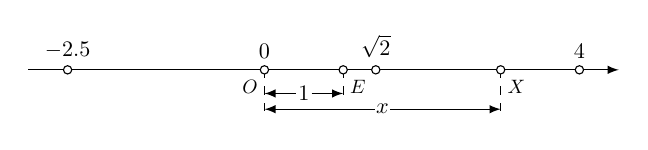
\begin{tikzpicture}
        \draw[-latex] (-3,0) -- (4.5,0);
        \draw[dashed] (0,0) -- (0,-0.6);
        \draw[dashed] (3,0) -- (3,-0.6);
        \draw[dashed] (1,0) -- (1,-0.4);

        \draw[-latex] (0.6,-0.3) -- (1,-0.3);
        \draw[-latex] (0.4,-0.3) -- (0,-0.3);
        \draw[-latex] (1.6,-0.5) -- (3,-0.5);
        \draw[-latex] (1.4,-0.5) -- (0,-0.5);

        \draw[fill=white] (0,0) circle (1.5pt)
        node[above,scale=0.8] at (0,0.05) {$0$}
        node[below left,scale=0.7] at (0,-0.05) {$O$};
        \draw[fill=white] (4,0) circle (1.5pt)
        node[above,scale=0.8] at (4,0.05) {$4$};
        \draw[fill=white] (-2.5,0) circle (1.5pt)
        node[above,scale=0.8] at (-2.5,0.05) {$-2.5$};
        \draw[fill=white] (1,0) circle (1.5pt)
        node[below right,scale=0.7] at (1,-0.05) {$E$};
        \draw[fill=white] (1.414,0) circle (1.5pt)
        node[above,scale=0.8] at (1.414,0.05) {$\sqrt{2}$};
        \draw[fill=white] (3,0) circle (1.5pt)
        node[below right,scale=0.7] at (3,-0.05) {$X$};

        \node[scale=0.8] at (0.5,-0.3) {$1$};
        \node[scale=0.8] at (1.5,-0.5) {$x$};
    \end{tikzpicture}
\end{figure}
则{\kaishu 这条直线上的任意一点 $X$ 必然对应于某一个实数 $x$,} 我们称其为该点的\emph{坐标}\index{zuobiao@坐标}(或横坐标).
若 $X$ 位于自 $O$ 起的正方向上, $x$ 即等于线段 $OX$ 的长度;
而在相反的情形下, 则等于这个长度的负值.

而由几何学上直线的连续性公理,
以点为集合的直线有类似于实数域连续性的性质 [\emph{\ref{subsec:10}}],
因此任意一个实数 $x$ 都必然对应于直线上的某一点.

这样, 在一切实数与有向直线(轴)上的点之间就可以建立起一一对应的关系.
实数可以被表示为轴上的点, 这条轴因此便被称为\emph{数轴}\index{shuzhou@数轴}.
